% Provenance (never printed): see sources/outline_sources.md (Year 1: vertical structure of
% the atmosphere, lapse rates, potential temperature and static stability; the layered
% ocean, the equation of state of seawater, T-S diagrams and water masses). Exercise and
% problem values in the Book 3 scratch calculator calc/ch26.py; figures from
% figdata/bachelor-1/atmosphere_profile.py (U.S. Standard Atmosphere 1976) and
% seawater_eos.py (EOS-80 and the UNESCO 44 algorithms; WOA23 columns, datasets
% bachelor-1-woa23-* and Book 2's grade-10-woa23-arctic-*).
% Physics owns the hydrostatic relation, the isothermal atmosphere and its scale height,
% the first law, Laplace's relation and Archimedes' thrust (recalled). Book 1 (g8) gave
% the layers and the environmental lapse rate of 6.5 K/km; Book 2 (g10) the dry adiabatic
% rate admitted, stable and unstable air, the mixed layer, thermocline, halocline and
% pycnocline: re-founded here with derivations. The moist adiabat is the Year 2 volume's.
\chapter{Estrutura da atmosfera e do oceano}\label{ch:b1:fluid-envelopes-structure}

Duas vezes por dia, em estações meteorológicas em todo o mundo, solta-se um balão que leva um
radiossonda, um pequeno instrumento que transmite por rádio a pressão, a temperatura e a umidade
do ar à medida que ele sobe; ele sobe a cerca de \qty{300}{m} por minuto e pode passar de
\qty{35}{km} antes que o balão estoure. Longe no mar, um navio de pesquisa baixa por um cabo, até
o abismo, um quadro de instrumentos e garrafas de água, medindo a condutividade, a temperatura e
a profundidade o tempo todo. Os dois perfis, um do ar e um da água, são a matéria-prima deste
capítulo. Os dois envelopes são estratificados, e em ambos a estratificação é fixada pela
densidade: fluido leve sobre fluido pesado. O que torna uma camada leve ou pesada é menos óbvio
do que parece. Ar mais frio que o ar abaixo dele pode ainda assim ser o mais leve; água mais
quente que a água acima dela pode ainda assim ser a mais pesada. O capítulo constrói as duas
ferramentas que resolvem isso, a \omterm{def:b1:fluid-envelopes-structure:potential-temperature}{temperatura potencial} e a \omterm{def:b1:fluid-envelopes-structure:eos}{equação de estado da água do mar}.
% ledger: nws:radiosonde, nws:radiosonde-def, commons:ctd-rosette

\begin{omfigure}
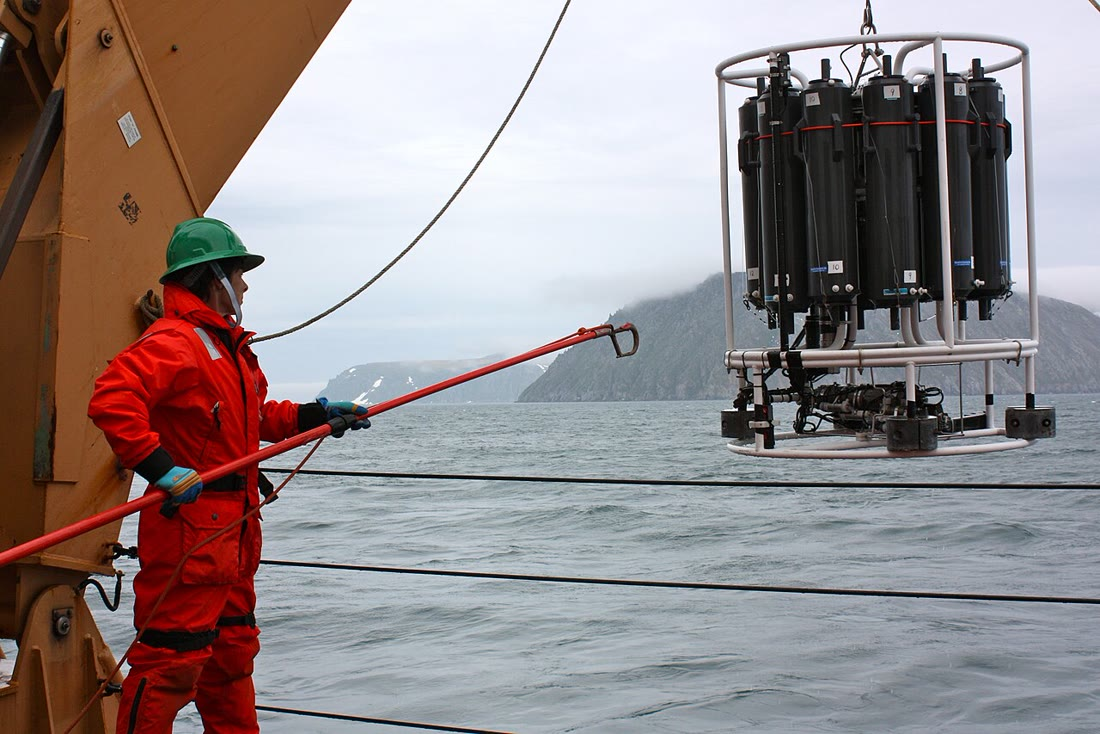
\includegraphics[width=0.62\linewidth]{images/book3/b1-ctd-rosette.jpg}

{\small Um CTD e uma roseta sendo trazidos a bordo no Estreito de Bering em junho de 2011. As
garrafas cinzentas em volta do quadro são fechadas em profundidades escolhidas na subida para
amostrar a água; os instrumentos na base do quadro medem a condutividade (da qual se calcula a
salinidade), a temperatura e a profundidade (na verdade a pressão) continuamente enquanto o
quadro desce. (NASA Goddard Space Flight Center, domínio público, via Wikimedia Commons.)}
\label{fig:b1:fluid-envelopes-structure:ctd}
\end{omfigure}
% ledger: commons:ctd-rosette, unesco44:atg-theta

\begin{recall}
Os livros de física dão a relação hidrostática, $\mathrm dp/\mathrm dz =
-\rho g$, para um fluido em repouso; para um gás ideal de massa molar $M$, $p = \rho R
T/M$, e em uma atmosfera isotérmica a pressão cai como $e^{-z/H}$ com a altura de escala
$H = RT/(Mg)$. Eles enunciam a primeira lei para um sistema fechado e, para um gás ideal, a
relação de Laplace ao longo de uma transformação adiabática reversível, $pV^{\gamma} = $
constante, com $\gamma = c_p/c_v$ e $c_p - c_v
= R/M$ por unidade de massa. Um corpo imerso em um fluido recebe um empuxo para cima igual
ao peso do fluido que desloca (Arquimedes). O Livro~1 nomeou as camadas da atmosfera e o
\omterm{def:b1:fluid-envelopes-structure:lapse-rate}{gradiente ambiental} da \omterm{def:b1:fluid-envelopes-structure:standard-atmosphere}{atmosfera padrão}, de \qty{6.5}{\celsius} por quilômetro na troposfera; o
Livro~2 admitiu o \omterm{def:b1:fluid-envelopes-structure:lapse-rate}{gradiente adiabático seco}, de \qty{9.8}{\celsius} por quilômetro, chamou o ar
de estável ou instável conforme o destino de uma porção empurrada para cima, e descreveu a
\omterm{def:b1:fluid-envelopes-structure:ocean-layers}{camada de mistura}, a \omterm{def:b1:fluid-envelopes-structure:ocean-layers}{termoclina}, a \omterm{def:b1:fluid-envelopes-structure:ocean-layers}{haloclina} e a \omterm{def:b1:fluid-envelopes-structure:ocean-layers}{picnoclina} do oceano. A salinidade da água do
mar é próxima de 35 gramas de sais dissolvidos por quilograma.
% ledger: ussa76:layers, nws:dalr, nos:salinity
\end{recall}

\section{Estrutura vertical da atmosfera}\label{sec:b1:fluid-envelopes-structure:atmosphere}

Nenhuma sondagem real é igual à seguinte. Para compará-las, um perfil de referência é fixado por
convenção.

\begin{definition}[Atmosfera padrão]\label{def:b1:fluid-envelopes-structure:standard-atmosphere}
Uma \emph{atmosfera padrão}\index{atmosfera padrão} é um perfil de temperatura, pressão e
densidade em função da altura fixado por convenção: ar seco de massa molar constante, um gás
ideal em equilíbrio hidrostático, com valores dados ao nível do mar e uma temperatura que varia
linearmente com a altura em camadas sucessivas. A atmosfera padrão de 1976 toma
\qty{288.15}{K} e \qty{101325}{Pa} ao nível do mar, $M_0 = \qty{28.9644}{kg.kmol^{-1}}$,
$R^* = \qty{8314.32}{J.kmol^{-1}.K^{-1}}$ e $g_0 = \qty{9.80665}{m.s^{-2}}$.
\end{definition}
% ledger: ussa76:sea-level

Abaixo de \qty{47}{km} a padrão de 1976 tem quatro camadas
(\cref{tab:b1:fluid-envelopes-structure:layers}). A mais baixa, a troposfera, esfria a
\qty{6.5}{K} por quilômetro; de seu topo, a tropopausa, a temperatura se mantém em
\qty{216.65}{K} por nove quilômetros, depois sobe. As alturas da padrão são alturas
geopotenciais, as alturas que uma gravidade constante $g_0$ daria à mesma energia potencial;
abaixo de \qty{32}{km} elas diferem das alturas geométricas em menos de \qty{0.6}{\percent} (os
\qty{11}{km} da padrão ficam a \qty{11.02}{km}).
% ledger: ussa76:layers, ussa76:sea-level

\begin{table}[ht]
\centering
\small
\renewcommand{\arraystretch}{1.2}
\begin{tabular}{|l|c|c|c|c|}
\hline
Camada & Base (km) & $\mathrm dT/\mathrm dz$ (K/km) & $T$ na base (K) & $p$ na base (hPa) \\
\hline
1 (troposfera) & 0 & $-6.5$ & 288.15 & 1013.25 \\
2 (estratosfera) & 11 & 0.0 & 216.65 & 226.32 \\
3 (estratosfera) & 20 & $+1.0$ & 216.65 & 54.75 \\
4 (estratosfera) & 32 & $+2.8$ & 228.65 & 8.68 \\
\hline
\end{tabular}
\caption{As quatro camadas mais baixas da \omterm{def:b1:fluid-envelopes-structure:standard-atmosphere}{atmosfera padrão} de 1976. Os gradientes e os valores
ao nível do mar são valores que definem a padrão; as temperaturas e pressões nas bases são
calculadas a partir deles com \cref{prop:b1:fluid-envelopes-structure:layer-pressure}.}
\label{tab:b1:fluid-envelopes-structure:layers}
\end{table}
% ledger: ussa76:layers, ussa76:sea-level (bases computed in figdata/bachelor-1/atmosphere_profile.py)

Em cada camada a temperatura é uma função linear da altura, de modo que a relação hidrostática
pode ser integrada em forma fechada.

\begin{proposition}[Pressão em uma camada de gradiente constante]\label{prop:b1:fluid-envelopes-structure:layer-pressure}
Em uma camada de ar seco onde $T = T_b - L\,(z - z_b)$ com $L \neq 0$ constante, a pressão é
\[
  p = p_b \left(\frac{T}{T_b}\right)^{gM/(RL)},
\]
onde $T_b$ e $p_b$ são os valores na base $z_b$. Quando $L = 0$ a pressão cai exponencialmente
com a altura de escala $H = RT_b/(Mg)$.
\end{proposition}

\begin{proof}
A relação hidrostática e o gás ideal dão $\mathrm dp/p = -(gM/R)\,\mathrm
dz/T$. Como $\mathrm dT = -L\,\mathrm dz$, isto é $\mathrm dp/p =
(gM/(RL))\,\mathrm dT/T$, que integra a $\ln(p/p_b) = (gM/(RL))
\ln(T/T_b)$. Para $L = 0$, $T = T_b$ e $\ln(p/p_b) = -(z - z_b)/H$: a
atmosfera isotérmica dos livros de física.
\end{proof}

Na troposfera da padrão, $gM/(RL) = 9.80665 \times 28.9644 /
(8314.32 \times 0.0065) = 5.256$, e a \qty{11}{km}, $T = 216.65$~K:
$p = \num{101325} \times (216.65/288.15)^{5.256} = \qty{22632}{Pa}$, um pouco
menos de um quarto do valor ao nível do mar. Na camada isotérmica acima, $H =
8314.32 \times 216.65/(28.9644 \times 9.80665) = \qty{6.34}{km}$, e nove
quilômetros acima a pressão caiu por um fator adicional $e^{9/6.34} =
4.13$, para \qty{5475}{Pa}. Como a pressão em um nível é o peso, por unidade de
área, do ar acima dele, metade da massa da \omterm{def:b1:fluid-envelopes-structure:standard-atmosphere}{atmosfera padrão} fica abaixo de
\qty{5.5}{km} e nove décimos abaixo de \qty{16}{km}.
% ledger: ussa76:sea-level, ussa76:layers (values computed in figdata/bachelor-1/atmosphere_profile.py)

\section{Gradientes térmicos e temperatura potencial}\label{sec:b1:fluid-envelopes-structure:lapse}

\begin{definition}[Gradientes ambiental e adiabático seco]\label{def:b1:fluid-envelopes-structure:lapse-rate}
O \emph{gradiente ambiental}\index{gradiente ambiental} é $\Gamma =
-\mathrm dT/\mathrm dz$, a taxa com que a temperatura do ar em repouso diminui com a altura,
como uma sondagem a mede. O \emph{gradiente adiabático seco}\index{gradiente adiabático seco}
$\Gamma_d$ é a taxa com que a temperatura de uma \omterm{def:b1:fluid-envelopes-structure:parcel}{porção de ar} não saturado diminui à medida que
a porção é elevada.
\end{definition}
% ledger: nws:dalr

Uma taxa de gradiente é positiva quando a temperatura cai com a altura. As duas taxas são de
naturezas diferentes: a primeira descreve o estado da atmosfera em um instante; a segunda, a
transformação de um pedaço de ar que se move.

\begin{definition}[Porção de ar]\label{def:b1:fluid-envelopes-structure:parcel}
Uma \emph{porção de ar}\index{porção de ar} é um volume de ar seguido em seu movimento, pequeno o
bastante para ter uma única temperatura e pressão e não perturbar o ar em volta, grande o bastante
para manter sua identidade: não troca massa e, durante um deslocamento rápido, nenhum calor com o
entorno, e sua pressão é a cada instante a do ar circundante.
\end{definition}

A porção é uma idealização, como o sistema fechado da termodinâmica: os resultados a seguir valem
para o ar real na medida em que um pedaço em movimento troca pouco calor e pouca massa com o
entorno.

\begin{theorem}[O gradiente adiabático seco]\label{thm:b1:fluid-envelopes-structure:dry-adiabatic}
Uma \omterm{def:b1:fluid-envelopes-structure:parcel}{porção de ar} seco, elevada adiabática e reversivelmente através de ar em repouso de
temperatura quase igual, esfria à taxa
\[
  \Gamma_d = \frac{g}{c_p},
\]
onde $c_p$ é o calor específico do ar a pressão constante. Com $c_p =
\qty{1004.7}{J.kg^{-1}.K^{-1}}$, $\Gamma_d = \qty{9.76}{K.km^{-1}}$.
\end{theorem}

\begin{proof}
Para um quilograma da porção, de temperatura $T_p$ e densidade $\rho_p$, a primeira lei de uma
transformação reversível sem troca de calor, escrita com a entalpia, é $c_p\,\mathrm dT_p - \mathrm dp/\rho_p = 0$. A pressão da porção é a do ar em volta, que é hidrostática: $\mathrm dp = -\rho_e
g\,\mathrm dz$, com $\rho_e$ a densidade do ar circundante. Logo
\[
  \frac{\mathrm dT_p}{\mathrm dz} = -\frac{g}{c_p}\,\frac{\rho_e}{\rho_p}
  = -\frac{g}{c_p}\,\frac{T_p}{T_e},
\]
já que, à mesma pressão, as densidades de dois gases ideais de mesma massa molar estão na razão
inversa de suas temperaturas. Quando a porção está quase à temperatura de seu entorno,
$T_p/T_e \approx 1$ e $-\mathrm dT_p/\mathrm dz
= g/c_p$. Para o ar seco, um gás diatômico ideal, $\gamma = 1.4$, logo $c_p =
\gamma/(\gamma - 1) \times R/M = 3.5 \times 8314.32/28.9644 =
\qty{1004.7}{J.kg^{-1}.K^{-1}}$, e $\Gamma_d = 9.80665/1004.7 =
\qty{0.00976}{K.m^{-1}}$.
\end{proof}
% ledger: nasa:grc-gamma, ussa76:sea-level, nws:dalr

Uma porção \qty{10}{K} mais quente que seu entorno, perto de \qty{280}{K}, esfria a
$\Gamma_d \times 290/280$, \qty{3.6}{\percent} mais depressa; a correção é desprezada no que
segue. A taxa não depende da pressão nem da temperatura da porção, e uma porção que afunda aquece
à mesma taxa, como o Livro~2 acompanhou o ar sobre uma montanha.

Integrar a mesma equação sem o passo hidrostático dá uma quantidade que a porção carrega consigo.

\begin{proposition}[Temperatura potencial]\label{prop:b1:fluid-envelopes-structure:theta}
Ao longo de uma transformação adiabática reversível do ar seco,
\[
  \theta = T\left(\frac{p_0}{p}\right)^{\kappa},\qquad \kappa = \frac{R}{Mc_p} =
  \frac{\gamma - 1}{\gamma} = \frac{2}{7},
\]
permanece constante, qualquer que seja a pressão de referência $p_0$.
\end{proposition}

\begin{proof}
A partir de $c_p\,\mathrm dT = \mathrm dp/\rho$ e $\rho = pM/(RT)$, $c_p\,\mathrm dT/T
= (R/M)\,\mathrm dp/p$, logo $\ln T - \kappa \ln p$ é constante, e também $T
p^{-\kappa}$; multiplicando pela constante $p_0^{\kappa}$ obtém-se $\theta$. Esta é
a relação de Laplace escrita com $T$ e $p$.
\end{proof}

\begin{definition}[Temperatura potencial]\label{def:b1:fluid-envelopes-structure:potential-temperature}
A \emph{temperatura potencial}\index{temperatura potencial} $\theta$ de uma \omterm{def:b1:fluid-envelopes-structure:parcel}{porção de ar} seco é a
temperatura que ela teria se trazida adiabaticamente à pressão de referência $p_0 = \qty{1000}{hPa}$:
$\theta = T\,(1000/p)^{2/7}$ com $p$ em hectopascais e $T$ em kelvins.
\end{definition}
% ledger: nws:potential-temperature

A \omterm{def:b1:fluid-envelopes-structure:potential-temperature}{temperatura potencial} é um rótulo que uma porção seca conserva quando sobe ou desce sem trocar
calor, como a salinidade de uma porção de água. O aquecimento por radiação, a condensação da água
ou a mistura a muda; o resto não.

\begin{example}[A tropopausa da atmosfera padrão]\label{ex:b1:fluid-envelopes-structure:tropopause}
Na superfície da padrão, $\theta = 288.15 \times (1000/1013.25)^{2/7} =
\qty{287.07}{K}$. Na tropopausa, $T = \qty{216.65}{K}$ e $p =
\qty{226.32}{hPa}$: $\theta = 216.65 \times (1000/226.32)^{2/7} = 216.65 \times
1.529 = \qty{331.2}{K}$. Ar da tropopausa trazido adiabaticamente para \qty{1000}{hPa} chegaria a
\qty{331.2}{K}, \qty{44}{K} mais quente que o ar da superfície trazido à mesma pressão. A
temperatura cai \qty{71.5}{K} do solo até a tropopausa, mas a \omterm{def:b1:fluid-envelopes-structure:potential-temperature}{temperatura potencial} sobe
\qty{44}{K}.
\end{example}
% ledger: ussa76:layers, nws:potential-temperature (values computed in figdata/bachelor-1/atmosphere_profile.py)

\section{Estabilidade estática}\label{sec:b1:fluid-envelopes-structure:stability}

\begin{definition}[Estabilidade estática; inversão de temperatura]\label{def:b1:fluid-envelopes-structure:stability}
A \emph{estabilidade estática}\index{estabilidade estática} de uma camada em repouso é sua resposta
a um pequeno deslocamento vertical de uma porção. A camada tem uma \emph{estratificação
estável}\index{estratificação estável} se a porção deslocada é empurrada de volta para seu nível,
uma \emph{estratificação instável}\index{estratificação instável} se é empurrada ainda mais para
longe, e uma \emph{estratificação neutra}\index{estratificação neutra} se nenhuma força age sobre
ela. Uma \emph{inversão de temperatura}\index{inversão de temperatura} é uma camada em que a
temperatura aumenta com a altura.
\end{definition}
% ledger: nws:inversion

\begin{theorem}[O critério da estabilidade estática]\label{thm:b1:fluid-envelopes-structure:stability}
Uma camada de ar seco em repouso, de temperatura $T$ e \omterm{def:b1:fluid-envelopes-structure:lapse-rate}{gradiente ambiental} $\Gamma$, é estável se
$\Gamma < \Gamma_d$, neutra se $\Gamma = \Gamma_d$ e instável se $\Gamma > \Gamma_d$; de modo
equivalente, é estável se e somente se sua \omterm{def:b1:fluid-envelopes-structure:potential-temperature}{temperatura potencial} aumenta com a altura. Uma porção
deslocada de uma pequena $\delta z$ em uma camada estável oscila em torno de seu nível à
frequência angular $N$, em que
\[
  N^2 = \frac{g}{T}\,(\Gamma_d - \Gamma) = \frac{g}{\theta}\,\frac{\mathrm d\theta}{\mathrm dz}.
\]
\end{theorem}

\begin{proof}
Uma porção à temperatura $T$ de seu nível é elevada de $\delta z$. Ela chega a $T - \Gamma_d\,\delta z$,
enquanto o ar em volta está em $T - \Gamma\,\delta z$. Por unidade de massa, a porção sente seu
peso e o empuxo de Arquimedes, uma aceleração ascendente líquida $g\,(\rho_e - \rho_p)/\rho_p = g\,(T_p - T_e)/T_e$, sendo as pressões iguais. Até primeira ordem em $\delta z$ isto é
\[
  \frac{\mathrm d^2 \delta z}{\mathrm dt^2} = -\frac{g}{T}\,(\Gamma_d - \Gamma)\,\delta z = -N^2\,\delta z .
\]
Se $\Gamma < \Gamma_d$, $N^2 > 0$ e a porção oscila à frequência angular $N$; se $\Gamma > \Gamma_d$
o deslocamento cresce exponencialmente; se $\Gamma = \Gamma_d$ nenhuma força age. Para a segunda
forma, tome a derivada logarítmica de $\theta = T (p_0/p)^{\kappa}$ e use a relação hidrostática:
\[
  \frac{1}{\theta}\frac{\mathrm d\theta}{\mathrm dz} = \frac{1}{T}\frac{\mathrm dT}{\mathrm dz}
  - \frac{\kappa}{p}\frac{\mathrm dp}{\mathrm dz} = -\frac{\Gamma}{T} + \frac{\kappa\,\rho g}{p}
  = -\frac{\Gamma}{T} + \frac{\kappa g M}{RT} = \frac{\Gamma_d - \Gamma}{T},
\]
pois $\kappa M/R = 1/c_p$.
\end{proof}

A frequência angular $N$ chama-se frequência de flutuabilidade. Na troposfera da padrão, perto do
solo, $N^2 = (9.80665/288.15) \times (9.761 -
6.5)\times10^{-3} = \qty{1.11e-4}{s^{-2}}$, $N = \qty{0.0105}{s^{-1}}$, e o período
$2\pi/N$ da oscilação é de cerca de \qty{10}{min}. Na estratosfera inferior isotérmica
$\Gamma = 0$: $N = \qty{0.0210}{s^{-1}}$, o dobro, com período de cinco minutos. A estratosfera é
uma tampa: resiste ao movimento vertical muito mais fortemente que a troposfera abaixo dela.
% ledger: ussa76:layers (values computed in figdata/bachelor-1/atmosphere_profile.py)

\begin{omfigure}
\begin{tikzpicture}
\begin{axis}[name=tz, omrecord, width=0.46\linewidth, height=7.2cm, xmin=160, xmax=300,
  ymin=0, ymax=32, xlabel={temperatura (K)}, ylabel={altura (km)}, xtick={160,200,...,300},
  ytick={0,5,...,30}]
% figdata/bachelor-1/atmosphere_profile.py; ledger: ussa76:sea-level, ussa76:layers, nasa:grc-gamma
\addplot[omDef, line width=0.9pt] table[x=T_K, y=z_km] {figdata/out/bachelor-1-atmosphere_profile-profile.dat};
\addplot[omThm, dashed, line width=0.7pt] table[x=T_K, y=z_km] {figdata/out/bachelor-1-atmosphere_profile-adiabat.dat};
\addplot[only marks, mark=*, mark size=1.6pt, black] table[x=T_K, y=z_km] {figdata/out/bachelor-1-atmosphere_profile-tropo.dat};
\node[font=\scriptsize, text=omThm, anchor=west, align=left] at (axis cs:163,17.0) {adiabática seca\\a partir da superfície};
\node[font=\scriptsize, text=omDef, anchor=west] at (axis cs:252,6.4) {padrão};
\node[font=\scriptsize, anchor=east] at (axis cs:214.5,11.9) {tropopausa};
\end{axis}
\begin{axis}[at={(tz.east)}, anchor=west, xshift=1.3cm, omrecord, width=0.46\linewidth, height=7.2cm,
  xmin=250, xmax=900, ymin=0, ymax=32, xlabel={temperatura potencial (K)}, ylabel={altura (km)},
  xtick={300,500,700,900}, ytick={0,5,...,30}]
\addplot[omDef, line width=0.9pt] table[x=theta_K, y=z_km] {figdata/out/bachelor-1-atmosphere_profile-profile.dat};
\addplot[only marks, mark=*, mark size=1.6pt, black] table[x=theta_K, y=z_km] {figdata/out/bachelor-1-atmosphere_profile-tropo.dat};
\node[font=\scriptsize, anchor=west] at (axis cs:345,10.2) {\num{331} K};
\end{axis}
\end{tikzpicture}

{\small A \omterm{def:b1:fluid-envelopes-structure:standard-atmosphere}{atmosfera padrão} de 1976 até \qty{32}{km}. À esquerda: temperatura, com a adiabática
seca que uma porção elevada a partir da superfície seguiria (tracejada). A \omterm{def:b1:fluid-envelopes-structure:standard-atmosphere}{atmosfera padrão} esfria mais
devagar que a adiabática, de modo que é estável em toda parte. À direita: \omterm{def:b1:fluid-envelopes-structure:potential-temperature}{temperatura potencial},
que sobe com a altura em toda parte, suavemente na troposfera e bruscamente acima da tropopausa
(ponto).}
\label{fig:b1:fluid-envelopes-structure:theta}
\end{omfigure}
% ledger: ussa76:sea-level, ussa76:layers, nasa:grc-gamma, nws:potential-temperature

Em um diagrama de temperatura contra altura, o critério compara duas inclinações (figura abaixo):
a porção segue a adiabática seca por seu ponto de partida, e a questão é de que lado da sondagem
ela se encontra após um pequeno deslocamento.

\begin{omfigure}
\begin{tikzpicture}[x=0.55cm, y=0.55cm, >={Stealth[length=2mm]}]
\foreach \dx/\envtop/\verdict in {0/-0.8/{camada estável: a porção afunda de volta}, 9/-3.8/{camada instável: a porção continua subindo}} {
  \begin{scope}[xshift=\dx cm]
  \draw[->] (0,0) -- (7.2,0) node[below left, font=\scriptsize] {temperatura};
  \draw[->] (0,0) -- (0,6.4) node[above right, font=\scriptsize] {altura};
  % sounding (environment): solid; dry adiabat through the starting point P: dashed
  \draw[omDef, line width=0.9pt] (5.0,0.6) -- (5.0+\envtop,5.4);
  \draw[omThm, dashed, line width=0.8pt] (5.0,0.6) -- (2.6,5.4);
  \fill (5.0,0.6) circle (2pt) node[right, font=\scriptsize] {$P$};
  \draw[densely dotted] (0,4.2) node[left, font=\scriptsize] {$z + \delta z$} -- (7,4.2);
  \fill[omThm] (3.2,4.2) circle (1.8pt);
  \fill[omDef] ({5.0+\envtop*3.6/4.8},4.2) circle (1.8pt);
  \node[font=\scriptsize, anchor=north] at (3.6,-0.5) {\verdict};
  \end{scope}
}
\end{tikzpicture}

{\small O método da porção. Azul contínuo: a sondagem; vermelho tracejado: a adiabática seca por
$P$. Uma porção começa em $P$ à temperatura do ar em volta e é elevada até $z + \delta z$ ao longo
da adiabática seca (ponto vermelho); a sondagem dá a temperatura do ar ali (ponto azul). À
esquerda: a sondagem esfria mais devagar que a adiabática; a porção chega mais fria, logo mais
densa, que seu entorno, e afunda de volta. À direita: a sondagem esfria mais depressa que a
adiabática; a porção chega mais quente e continua subindo.}
\label{fig:b1:fluid-envelopes-structure:parcel}
\end{omfigure}

\begin{method}[Lendo a estabilidade de uma sondagem]\label{met:b1:fluid-envelopes-structure:sounding}
\begin{enumerate}
  \item Divida a sondagem em camadas entre níveis onde a inclinação muda.
  \item Em cada camada calcule $\Gamma = -(T_2 - T_1)/(z_2 - z_1)$, em kelvins por quilômetro.
  \item Compare com $\Gamma_d = \qty{9.8}{K/km}$: $\Gamma > \Gamma_d$ instável, $\Gamma$ próximo
        de $\Gamma_d$ neutro, $\Gamma < \Gamma_d$ estável; um $\Gamma$ negativo é uma inversão, o
        caso mais estável.
  \item Onde as pressões são dadas em vez das alturas, calcule $\theta =
        T(1000/p)^{2/7}$ em cada nível: $\theta$ decrescendo para cima marca uma camada instável,
        constante uma neutra, crescente uma estável.
\end{enumerate}
\end{method}

Uma camada instável não dura: um deslocamento nela cresce exponencialmente, à taxa
$\sqrt{-N^2}$, e as porções que ela libera a viram, misturando-a até que sua \omterm{def:b1:fluid-envelopes-structure:potential-temperature}{temperatura
potencial} seja uniforme e seu gradiente seja $\Gamma_d$. Uma camada aquecida por baixo, pelo solo
quente ou por um mar quente, é empurrada para a instabilidade; uma resfriada por baixo, para a
estabilidade. Uma inversão limita tudo o que está abaixo dela: uma porção que sobe de baixo se
encontra mais fria que seu entorno assim que entra nela. Acima de \qty{20}{km} toda a
estratosfera da padrão é uma inversão.

Tudo isso supõe ar seco. Uma porção em elevação que se satura libera calor latente à medida que
sua água condensa, e esfria mais devagar que $\Gamma_d$; a adiabática saturada e a instabilidade
condicional que ela traz são assunto do volume do próximo ano.
% ledger: nws:inversion, nws:dalr

\section{O oceano estratificado}\label{sec:b1:fluid-envelopes-structure:ocean}

O oceano troca calor e água com a atmosfera apenas em sua superfície, por aquecimento e
resfriamento, evaporação e chuva. Sua estrutura vertical tem três ingredientes: temperatura,
salinidade e densidade.

\begin{definition}[Camada de mistura, termoclina, haloclina, picnoclina]\label{def:b1:fluid-envelopes-structure:ocean-layers}
A \emph{camada de mistura}\index{camada de mistura} é a camada superficial do oceano cuja
temperatura, salinidade e densidade são quase uniformes com a profundidade; sua profundidade é
lida em um perfil como a profundidade onde a temperatura se afasta pela primeira vez de seu valor
de superfície de um limiar escolhido, em geral \qty{0.5}{\celsius}. A \emph{termoclina}\index{termoclina},
a \emph{haloclina}\index{haloclina} e a \emph{picnoclina}\index{picnoclina} são as camadas abaixo
dela em que a temperatura, a salinidade e a densidade, respectivamente, mudam mais depressa com a
profundidade.
\end{definition}

A pressão no oceano é dada em decibares, porque um decibar, \qty{e4}{Pa}, é quase a pressão de um
metro de água do mar: a \qty{30}{\degree} de \omterm{def:b1:spherical-astronomy:geographic}{latitude}, \qty{1000}{dbar} ficam a \qty{990.8}{m} e
\qty{10000}{dbar} a \qty{9712.7}{m}.
% ledger: unesco:eos80-checks (DEPTH table computed in figdata/bachelor-1/seawater_eos.py)

A água é quase incompressível, mas não totalmente, e uma porção de água trazida das
profundezas se expande e esfria um pouco, como uma \omterm{def:b1:fluid-envelopes-structure:parcel}{porção de ar}. A taxa adiabática da água do
mar é pequena, cerca de \qty{0.04}{\celsius} por \qty{1000}{dbar} na superfície a
\qty{0}{\celsius} e \qty{0.09}{\celsius} por \qty{1000}{dbar} a \qty{3000}{dbar}, contra \num{9.8}
por quilômetro no ar; mas em cinco quilômetros ela soma algumas décimas de grau, mais que as
diferenças entre as águas profundas. Oceanógrafos comparam, portanto, as águas também por sua
temperatura \emph{potencial}: a temperatura que uma porção teria se elevada adiabaticamente, sem
mudança de salinidade, até a superfície. Uma água de \qty{2}{\celsius} a \qty{4000}{dbar} e
salinidade 35 tem uma \omterm{def:b1:fluid-envelopes-structure:potential-temperature}{temperatura potencial} de \qty{1.66}{\celsius}. Nos níveis mais profundos do
Atlântico Sul a \qty{10.5}{\degree S}, a temperatura medida sobe de \qty{0.730}{\celsius} a
\qty{5400}{m} para \qty{0.731}{\celsius} a \qty{5500}{m} enquanto a \omterm{def:b1:fluid-envelopes-structure:potential-temperature}{temperatura potencial} cai de
\qty{0.261}{\celsius} para \qty{0.250}{\celsius}: o aquecimento é compressão, não calor.
% ledger: unesco44:atg-theta, data:b3-woa23 (values computed in figdata/bachelor-1/seawater_eos.py)

\begin{omfigure}
\begin{tikzpicture}
\begin{groupplot}[group style={group size=3 by 1, horizontal sep=0.55cm, yticklabels at=edge left},
  omrecord, omdepth, width=0.365\linewidth, height=7.4cm, ymin=0, ymax=2000,
  ytick={0,500,1000,1500,2000}, y tick label style={/pgf/number format/.cd, set thousands separator={}},
  every axis label/.append style={font=\small}]
\nextgroupplot[xmin=-2, xmax=28, xlabel={$\theta$ (\si{\celsius})}, ylabel={profundidade (m)}, xtick={0,10,20}]
% figdata/bachelor-1/seawater_eos.py; WOA23 (datasets bachelor-1-woa23-*, grade-10-woa23-arctic-*); ledger: data:b3-woa23, data:b2-woa23, unesco44:atg-theta
\addplot[omThm, line width=0.8pt] table[x=theta, y=depth] {figdata/out/bachelor-1-seawater_eos-prof-sa10.dat};
\addplot[omProp, line width=0.8pt] table[x=theta, y=depth] {figdata/out/bachelor-1-seawater_eos-prof-sa30.dat};
\addplot[omDef, line width=0.8pt] table[x=theta, y=depth] {figdata/out/bachelor-1-seawater_eos-prof-arctic.dat};
\draw[omThm, line width=0.8pt] (axis cs:9,1250) -- (axis cs:13,1250) node[right, font=\scriptsize, text=black] {\qty{10.5}{\degree S}};
\draw[omProp, line width=0.8pt] (axis cs:9,1450) -- (axis cs:13,1450) node[right, font=\scriptsize, text=black] {\qty{30.5}{\degree S}};
\draw[omDef, line width=0.8pt] (axis cs:9,1650) -- (axis cs:13,1650) node[right, font=\scriptsize, text=black] {\qty{75.5}{\degree N}};
\nextgroupplot[xmin=28, xmax=37.5, xlabel={salinidade}, xtick={28,31,34,37}]
\addplot[omThm, line width=0.8pt] table[x=s, y=depth] {figdata/out/bachelor-1-seawater_eos-prof-sa10.dat};
\addplot[omProp, line width=0.8pt] table[x=s, y=depth] {figdata/out/bachelor-1-seawater_eos-prof-sa30.dat};
\addplot[omDef, line width=0.8pt] table[x=s, y=depth] {figdata/out/bachelor-1-seawater_eos-prof-arctic.dat};
\nextgroupplot[xmin=22, xmax=28.5, xlabel={$\sigma_\theta$ (\si{kg.m^{-3}})}, xtick={22,24,26,28}]
\addplot[omThm, line width=0.8pt] table[x=sigma, y=depth] {figdata/out/bachelor-1-seawater_eos-prof-sa10.dat};
\addplot[omProp, line width=0.8pt] table[x=sigma, y=depth] {figdata/out/bachelor-1-seawater_eos-prof-sa30.dat};
\addplot[omDef, line width=0.8pt] table[x=sigma, y=depth] {figdata/out/bachelor-1-seawater_eos-prof-arctic.dat};
\end{groupplot}
\end{tikzpicture}

{\small \omterm{def:b1:fluid-envelopes-structure:potential-temperature}{Temperatura potencial}, salinidade e \omterm{def:b1:fluid-envelopes-structure:eos}{anomalia de densidade} potencial
(\cref{def:b1:fluid-envelopes-structure:eos}) nos \qty{2000}{m} superiores, na média anual, em
três lugares: o Atlântico Sul tropical (\qty{10.5}{\degree S}, \qty{25.5}{\degree W}), o Atlântico
Sul subtropical (\qty{30.5}{\degree S}, \qty{25.5}{\degree W}) e a Bacia do Canadá, no oceano
Ártico (\qty{75.5}{\degree N}, \qty{150.5}{\degree W}). Dados: World Ocean Atlas 2023.}
\label{fig:b1:fluid-envelopes-structure:profiles}
\end{omfigure}
% ledger: data:b3-woa23, data:b2-woa23, unesco:eos80, unesco44:atg-theta

As três colunas da figura acima mostram os três tipos de oceano superior. Nos trópicos, uma
\omterm{def:b1:fluid-envelopes-structure:ocean-layers}{camada de mistura} quente perto de \qty{26.5}{\celsius} repousa sobre uma \omterm{def:b1:fluid-envelopes-structure:ocean-layers}{termoclina} nítida: entre
\qty{100}{m} e \qty{200}{m} a \omterm{def:b1:fluid-envelopes-structure:potential-temperature}{temperatura potencial} cai de \qty{24.0}{\celsius} para
\qty{14.4}{\celsius}, e a densidade a acompanha, de modo que a \omterm{def:b1:fluid-envelopes-structure:ocean-layers}{termoclina} é também a \omterm{def:b1:fluid-envelopes-structure:ocean-layers}{picnoclina}. A
\qty{30.5}{\degree S} a superfície é mais fria, \qty{21.1}{\celsius}, e a queda é mais gradual,
distribuída pelos \qty{800}{m} superiores. Nas duas, a salinidade é maior perto da superfície e
diminui para baixo; ela trabalha contra a estratificação, que a temperatura mais do que compensa.
A coluna do Ártico é o caso oposto. Sua água de superfície, a \qty{-1.4}{\celsius}, é a mais fria
das três, mas também a mais leve, $\sigma_\theta = 22.5$, porque sua salinidade é de apenas
\num{28.1}; a salinidade sobe para \num{34.5} a \qty{300}{m}. A \omterm{def:b1:fluid-envelopes-structure:ocean-layers}{haloclina} é a \omterm{def:b1:fluid-envelopes-structure:ocean-layers}{picnoclina} aqui.
Abaixo dela há uma camada mais quente que a água acima, perto de \qty{0.7}{\celsius} a
\qty{475}{m}: uma \omterm{def:b1:fluid-envelopes-structure:stability}{inversão de temperatura} perfeitamente estável, mantida para baixo por seu sal.
% ledger: data:b3-woa23, data:b2-woa23 (values computed in figdata/bachelor-1/seawater_eos.py)

\section{Densidade da água do mar e diagramas T--S}\label{sec:b1:fluid-envelopes-structure:ts}

\begin{definition}[Equação de estado da água do mar; coeficiente de contração halina; anomalia de densidade]\label{def:b1:fluid-envelopes-structure:eos}
A \emph{equação de estado da água do mar}\index{equação de estado da água do mar} dá sua
densidade $\rho(S, T, p)$ em função da salinidade, da temperatura e da pressão. O
\emph{coeficiente de contração halina}\index{coeficiente de contração halina} é $\beta = (1/\rho)\,\partial\rho/\partial S$ a temperatura e pressão constantes. A
\emph{anomalia de densidade}\index{anomalia de densidade} $\sigma$ é uma densidade menos
\qty{1000}{kg.m^{-3}}: $\sigma_t = \rho(S, T, 0) -
1000$ usa a temperatura medida à pressão nula do mar, e a anomalia de densidade potencial
$\sigma_\theta = \rho(S, \theta, 0) - 1000$ usa a \omterm{def:b1:fluid-envelopes-structure:potential-temperature}{temperatura potencial}.
\end{definition}
% ledger: teos10:alpha-beta, teos10:sigma

A equação de estado não é derivada de primeiros princípios, mas ajustada a medidas de laboratório.
A equação internacional de 1980, na pressão da superfície, é um polinômio com quinze coeficientes,
$\rho = \rho_w(T) +
A(T)\,S + B(T)\,S^{3/2} + C\,S^2$, onde $\rho_w$ é a densidade da água pura; ela dá
$\rho(35, \qty{0}{\celsius}) = \qty{1028.1063}{kg.m^{-3}}$. Uma descrição termodinâmica da água do
mar, o TEOS-10, foi adotada em 2009 para substituí-la como a oficial; a equação de 1980 é usada aqui
porque seu polinômio cabe em uma página. Seu coeficiente de expansão térmica $\alpha = -(1/\rho)\,\partial\rho/\partial T$ é o coeficiente dos livros de física.
% ledger: unesco:eos80, teos10:alpha-beta, teos10:replaced

\begin{table}[ht]
\centering
\small
\renewcommand{\arraystretch}{1.2}
\begin{tabular}{|c|c|c|c|}
\hline
$T$ (\si{\celsius}) & $\rho(35, T, 0)$ (\si{kg.m^{-3}}) & $\alpha$ (\si{K^{-1}}) & $\beta$ \\
\hline
0 & 1028.106 & \num{0.53e-4} & \num{7.85e-4} \\
10 & 1026.952 & \num{1.67e-4} & \num{7.61e-4} \\
25 & 1023.343 & \num{2.97e-4} & \num{7.39e-4} \\
\hline
\end{tabular}
\caption{Densidade e coeficientes de expansão da água do mar de salinidade 35 à pressão da
superfície, pela equação internacional de estado de 1980.}
\label{tab:b1:fluid-envelopes-structure:density}
\end{table}
% ledger: unesco:eos80 (computed in figdata/bachelor-1/seawater_eos.py)

O coeficiente de expansão é seis vezes maior na água quente que na água perto do congelamento,
enquanto $\beta$ quase não muda (\cref{tab:b1:fluid-envelopes-structure:density}). Uma unidade de
salinidade pesa tanto quanto cerca de \qty{4.6}{\celsius} a \qty{10}{\celsius}, mas tanto quanto
\qty{15}{\celsius} perto de \qty{0}{\celsius}: na água polar fria, a densidade é fixada pela
salinidade, como mostrou a coluna do Ártico.

\begin{proposition}[Equação de estado linear]\label{prop:b1:fluid-envelopes-structure:linear-eos}
Perto de um estado de referência $(S_0, T_0)$ de densidade $\rho_0$, à pressão fixa,
\[
  \rho \approx \rho_0\bigl[1 - \alpha\,(T - T_0) + \beta\,(S - S_0)\bigr],
\]
com $\alpha$ e $\beta$ avaliados no estado de referência; o erro é de segunda ordem em
$T - T_0$ e $S - S_0$.
\end{proposition}

\begin{proof}
Esta é a expansão de Taylor de primeira ordem de $\rho(S, T)$ em $(S_0, T_0)$, já que
$\partial\rho/\partial T = -\rho_0\alpha$ e $\partial\rho/\partial S =
\rho_0\beta$ ali.
\end{proof}

Em torno de $(35, \qty{10}{\celsius})$ a forma linear dá a densidade da água em
$(35.2, \qty{11}{\celsius})$ a menos de \qty{0.01}{kg.m^{-3}}, mas a de uma água de superfície em
$(35.8, \qty{22.4}{\celsius})$ fica \qty{0.74}{kg.m^{-3}} alta demais: a equação de estado é
curva, e sua curvatura tem consequências.
% ledger: unesco:eos80 (computed in calc/ch26.py)

\begin{definition}[Diagrama T--S; massa de água]\label{def:b1:fluid-envelopes-structure:ts-diagram}
Um \emph{diagrama T--S}\index{diagrama T--S} é um gráfico da \omterm{def:b1:fluid-envelopes-structure:potential-temperature}{temperatura potencial} das amostras
de um perfil contra sua salinidade, com as profundidades escritas ao longo da curva e as retas de
igual $\sigma_\theta$ desenhadas por baixo. Uma \emph{massa de água}\index{massa de água} é um
corpo de água com uma história de formação comum, reconhecido por sua faixa de \omterm{def:b1:fluid-envelopes-structure:potential-temperature}{temperatura
potencial} e salinidade.
\end{definition}
% ledger: tomczak:water-masses

Uma \omterm{def:b1:fluid-envelopes-structure:ts-diagram}{massa de água} adquire sua temperatura e salinidade na superfície, por aquecimento e
resfriamento, evaporação e chuva, na região onde se forma; uma vez que afunda abaixo da \omterm{def:b1:fluid-envelopes-structure:ocean-layers}{camada de
mistura}, fora de contato com a atmosfera, só pode mudá-las misturando-se com seus vizinhos.
\omterm{def:b1:fluid-envelopes-structure:potential-temperature}{Temperatura potencial} e salinidade são então traçadores.

\begin{proposition}[Retas de mistura são retas]\label{prop:b1:fluid-envelopes-structure:mixing}
Quando massas $m_1$ e $m_2$ de duas águas $(S_1, \theta_1)$ e $(S_2, \theta_2)$ se misturam
completamente, a mistura tem
\[
  S = \frac{m_1 S_1 + m_2 S_2}{m_1 + m_2},\qquad
  \theta \approx \frac{m_1 \theta_1 + m_2 \theta_2}{m_1 + m_2}:
\]
em um \omterm{def:b1:fluid-envelopes-structure:ts-diagram}{diagrama T--S} ela fica sobre o segmento que une as duas águas, a distâncias delas na razão
inversa de suas massas. Misturas de três águas preenchem o triângulo que elas formam.
\end{proposition}

\begin{proof}
A salinidade é uma fração mássica de sal, e o sal se conserva: a massa de sal na mistura,
$m_1 S_1 + m_2 S_2$, dividida por sua massa, dá $S$. A mistura a pressão constante conserva a
entalpia; com um calor específico que varia pouco, isto é uma média ponderada das temperaturas
potenciais, a menos de um erro relativo de cerca de $3.4\times10^{-4}$ por unidade de diferença
de salinidade. O ponto $(S, \theta)$ é então o baricentro dos dois pontos com os pesos $m_1$ e
$m_2$.
\end{proof}
% ledger: teos10:mixing

\begin{omfigure}
\begin{tikzpicture}
\begin{axis}[omrecord, width=0.82\linewidth, height=9cm, xmin=33.5, xmax=37.4, ymin=-2, ymax=28,
  xlabel={salinidade}, ylabel={temperatura potencial (\si{\celsius})}, xtick={34,35,36,37},
  ytick={0,5,...,25}, x tick label style={/pgf/number format/.cd, fixed, precision=1}]
% figdata/bachelor-1/seawater_eos.py; ledger: unesco:eos80, unesco44:atg-theta, data:b3-woa23, tomczak:water-masses
\foreach \s in {24,25,26,26.5,27,27.5,28} {
  \addplot[black!35, line width=0.4pt] table[x=s, y=theta] {figdata/out/bachelor-1-seawater_eos-iso-\s.dat};
}
\addplot[only marks, mark=none, nodes near coords, point meta=explicit symbolic,
  every node near coord/.style={font=\scriptsize, text=black!55, anchor=west}]
  table[x=s, y=theta, meta=lab] {figdata/out/bachelor-1-seawater_eos-isolab.dat};
\addplot[omThm, line width=0.9pt] table[x=s, y=theta] {figdata/out/bachelor-1-seawater_eos-ts-sa10.dat};
\addplot[omProp, line width=0.9pt] table[x=s, y=theta] {figdata/out/bachelor-1-seawater_eos-ts-sa30.dat};
\addplot[only marks, mark=*, mark size=1.7pt, black] table[x=s, y=theta] {figdata/out/bachelor-1-seawater_eos-masses.dat};
\node[font=\scriptsize, anchor=south east] at (axis cs:35.5,15.6) {Água Central};
\node[font=\scriptsize, anchor=south east] at (axis cs:34.25,5.0) {AAIW};
\node[font=\scriptsize, anchor=west] at (axis cs:34.96,2.9) {NADW};
\node[font=\scriptsize, anchor=north] at (axis cs:34.70,0.5) {AABW};
\addplot[omDef, densely dashed, line width=0.7pt, mark=o, mark size=1.8pt] table[x=s, y=theta] {figdata/out/bachelor-1-seawater_eos-cabbeling.dat};
\node[font=\scriptsize, text=omDef, anchor=west] at (axis cs:34.98,7.6) {mistura};
\draw[omThm, line width=0.9pt] (axis cs:33.65,26.2) -- (axis cs:33.95,26.2) node[right, font=\scriptsize, text=black] {\qty{10.5}{\degree S}};
\draw[omProp, line width=0.9pt] (axis cs:33.65,24.7) -- (axis cs:33.95,24.7) node[right, font=\scriptsize, text=black] {\qty{30.5}{\degree S}};
\end{axis}
\end{tikzpicture}

{\small \omterm{def:b1:fluid-envelopes-structure:ts-diagram}{Diagrama T--S} das duas colunas do Atlântico Sul da figura de perfis, da superfície ao fundo
do mar, sobre retas de igual \omterm{def:b1:fluid-envelopes-structure:eos}{anomalia de densidade} potencial $\sigma_\theta$ (cinzas, rotuladas em
\si{kg.m^{-3}} em suas extremidades superiores). Pontos: os núcleos das \omterm{def:b1:fluid-envelopes-structure:ts-diagram}{massas de água} lidos na
coluna a \qty{30.5}{\degree S}. Azul: duas águas de mesma densidade, $\sigma_\theta = 27.0$, a
\qty{2}{\celsius} e \qty{14}{\celsius}, e sua mistura em partes iguais, sobre a reta que as une e
mais densa que ambas. Dados: World Ocean Atlas 2023.}
\label{fig:b1:fluid-envelopes-structure:ts}
\end{omfigure}
% ledger: data:b3-woa23, unesco:eos80, unesco44:atg-theta, tomczak:water-masses

As duas colunas do Atlântico Sul desenham a mesma figura no \omterm{def:b1:fluid-envelopes-structure:ts-diagram}{diagrama T--S}: a semelhança das curvas
de lugares distantes é o que revela as \omterm{def:b1:fluid-envelopes-structure:ts-diagram}{massas de água}. Da superfície até cerca de \qty{500}{m}, as
curvas seguem uma reta quase, íngreme em temperatura: é a Água Central, que preenche o quilômetro
superior do oceano subtropical. Abaixo dela, as duas curvas se voltam para um mínimo de salinidade,
\num{34.30} a \qty{900}{m} e \qty{4.3}{\celsius} a \qty{30.5}{\degree S}: a Água Intermediária
Antártica (AAIW), formada sob os ventos de oeste chuvosos do Oceano Austral, afundando até cerca de
\qty{1000}{m} e espalhando-se para o norte. Mais fundo, um máximo de salinidade, \num{34.90} a
\qty{2900}{m}: a Água Profunda do Atlântico Norte (NADW), formada nos mares da Groenlândia e de
Labrador, afundando até cerca de \qty{3000}{m} e movendo-se para o sul por todo o Atlântico. No
fundo as curvas convergem para a água mais fria, \qty{0.8}{\celsius} a \qty{4900}{m}: a Água de
Fundo Antártica (AABW), formada ao longo do continente antártico, que preenche os oceanos abaixo de
cerca de \qty{4000}{m}. A \qty{10.5}{\degree S} o mínimo de salinidade fica a \qty{750}{m} e o
máximo a \qty{1800}{m}, com um máximo mais alto, \num{34.95}: a NADW está mais perto de sua fonte ali.
% ledger: tomczak:water-masses, data:b3-woa23 (cores computed in figdata/bachelor-1/seawater_eos.py)

Os extremos são eles mesmos produtos de mistura. A AAIW, ao se mover para o norte, mistura-se com a
água mais salgada acima e abaixo dela; pela \cref{prop:b1:fluid-envelopes-structure:mixing} seu
núcleo se move em direção a elas no diagrama e o mínimo se erode. Um mínimo ou máximo de salinidade
em um perfil é sempre o rastro de uma água que veio de outro lugar, transportada lateralmente em
seu próprio nível de densidade.
% ledger: tomczak:water-masses

\begin{method}[Lendo massas de água em um diagrama T--S]\label{met:b1:fluid-envelopes-structure:ts}
\begin{enumerate}
  \item Converta as temperaturas medidas em temperaturas potenciais (no quilômetro superior a
        diferença é inferior a \qty{0.1}{\celsius} e pode ser desprezada).
  \item Plote $\theta$ contra $S$, escrevendo as profundidades ao longo da curva.
  \item Leia os segmentos retos como misturas das duas águas em suas extremidades, os extremos de
        salinidade ou de temperatura como núcleos de \omterm{def:b1:fluid-envelopes-structure:ts-diagram}{massas de água}, e o fim da curva perto do fundo
        como a água mais densa presente.
  \item Leia a densidade nas isopicnais: ao longo de um perfil estável, $\sigma_\theta$ aumenta
        com a profundidade.
\end{enumerate}
\end{method}

Como as isopicnais são curvas, duas águas de mesma densidade não se misturam em uma água dessa
densidade. Água em $(33.79, \qty{2}{\celsius})$ e água em $(36.05, \qty{14}{\celsius})$ têm ambas
$\sigma_\theta = 27.00$; misturadas em partes iguais, dão $(34.92, \qty{8}{\celsius})$, de
$\sigma_\theta = 27.21$ (figura acima). A mistura é mais densa que as duas águas que a originaram
e afunda abaixo delas.
Essa densificação na mistura, chamada cabbeling, é o preço da curvatura da equação de estado: com a
forma linear de \cref{prop:b1:fluid-envelopes-structure:linear-eos}, a densidade de uma mistura
seria a média das densidades. Ao longo das superfícies isopicnais do oceano, onde os redemoinhos
misturam águas de temperatura e salinidade diferentes, o cabbeling impele um afundamento lento
através delas.
% ledger: teos10:cabbeling, unesco:eos80 (example computed in figdata/bachelor-1/seawater_eos.py)

Uma última advertência. Referida à superfície, a AABW a \qty{30.5}{\degree S} resulta em
$\sigma_\theta = 27.854$, um pouco mais leve que a NADW acima dela, \num{27.857}; no fundo da
coluna a \qty{10.5}{\degree S}, $\sigma_\theta$ até diminui para baixo. A razão $\alpha/\beta$ da
equação de estado muda com a pressão, de modo que a ordem de duas águas de temperaturas diferentes
pode depender da pressão em que suas densidades são comparadas. Águas com milhares de metros de
profundidade são comparadas com uma densidade referida a uma pressão mais próxima da sua, como
$\sigma_2$, referida a \qty{2000}{dbar}; o método é o do volume do próximo ano.
% ledger: teos10:sigma, teos10:thermobaric, data:b3-woa23 (values computed in figdata/bachelor-1/seawater_eos.py)

\section{Exercícios}

\begin{exercise}[$\star$]\label{exo:b1:fluid-envelopes-structure:1}
(a)~Calcule a altura de escala do ar a \qty{250}{K} com as constantes da \omterm{def:b1:fluid-envelopes-structure:standard-atmosphere}{atmosfera padrão}.
(b)~Em que fator a pressão cai ao longo de \qty{10}{km} em uma camada isotérmica a essa
temperatura? (c)~Por que a altura de escala é menor na tropopausa que no solo?
% ledger: ussa76:sea-level
\end{exercise}

\begin{exercise}[$\star$]\label{exo:b1:fluid-envelopes-structure:2}
Uma sondagem dá, em kelvins por quilômetro, os gradientes $\Gamma = 11.0$
(\qtyrange{0}{0.3}{km}), $9.7$ (\qtyrange{0.3}{1.2}{km}), $-4.0$
(\qtyrange{1.2}{1.5}{km}), $6.0$ (\qtyrange{1.5}{8}{km}) e $0.0$ (acima de
\qty{8}{km}). Classifique cada camada como instável, neutra, estável ou uma inversão, e diga qual
é a mais estável.
% ledger: nws:dalr, nws:inversion
\end{exercise}

\begin{exercise}[$\star$]\label{exo:b1:fluid-envelopes-structure:3}
(a)~A água do mar tem densidade de \qty{1026.95}{kg.m^{-3}}. Qual é sua \omterm{def:b1:fluid-envelopes-structure:eos}{anomalia de densidade}?
(b)~De duas águas, A com $\sigma_\theta = 27.12$ e B com $\sigma_\theta = 26.78$, qual fica acima
da outra quando ambas estão em repouso na mesma coluna? (c)~Por que os oceanógrafos escrevem
$\sigma$ em vez de $\rho$?
% ledger: teos10:sigma
\end{exercise}

\begin{exercise}[$\star$]\label{exo:b1:fluid-envelopes-structure:4}
Água P $(S = 35.40, \theta = \qty{15.0}{\celsius})$ se mistura com a água Q $(S =
34.30, \theta = \qty{4.0}{\celsius})$. (a)~Calcule a salinidade e a \omterm{def:b1:fluid-envelopes-structure:potential-temperature}{temperatura potencial} de uma
mistura de uma parte de P com três partes de Q. (b)~Onde ela fica no \omterm{def:b1:fluid-envelopes-structure:ts-diagram}{diagrama T--S}?
(c)~Acrescenta-se uma terceira água R $(34.90,
\qty{2.5}{\celsius})$. A mistura das três pode ter $(34.60, \qty{8.0}{\celsius})$?
% ledger: teos10:mixing
\end{exercise}

\begin{exercise}[$\star\star$]\label{exo:b1:fluid-envelopes-structure:5}
(a)~A \qty{500}{hPa} o ar está a \qty{-20}{\celsius}. Calcule sua \omterm{def:b1:fluid-envelopes-structure:potential-temperature}{temperatura potencial}.
(b)~No solo, a \qty{1000}{hPa}, o ar está a \qty{25}{\celsius}. A camada entre os dois é estável
para ar seco? (c)~Qual seria a temperatura do ar de \qty{500}{hPa} trazido adiabaticamente ao solo?
% ledger: nws:potential-temperature
\end{exercise}

\begin{exercise}[$\star\star$]\label{exo:b1:fluid-envelopes-structure:6}
(a)~Com \cref{prop:b1:fluid-envelopes-structure:layer-pressure}, calcule a pressão a
\qty{5}{km} na \omterm{def:b1:fluid-envelopes-structure:standard-atmosphere}{atmosfera padrão}. (b)~Calcule-a de novo supondo uma atmosfera isotérmica a
\qty{288.15}{K}. Qual é menor, e por quê? (c)~Calcule a pressão a \qty{20}{km} a partir dos
valores a \qty{11}{km} de \cref{tab:b1:fluid-envelopes-structure:layers}.
% ledger: ussa76:sea-level, ussa76:layers
\end{exercise}

\begin{exercise}[$\star\star$]\label{exo:b1:fluid-envelopes-structure:7}
Use a equação de estado linear em torno de $(35, \qty{10}{\celsius})$ com os coeficientes de
\cref{tab:b1:fluid-envelopes-structure:density}. (a)~Que variação de salinidade compensa, para a
densidade, um aquecimento de \qty{1}{\celsius}? (b)~Uma água a \qty{10}{\celsius} é aquecida em
\qty{2}{\celsius} e tornada mais salgada em \num{0.3}. Ela fica mais densa ou mais leve, e de
quanto? (c)~Responda à mesma pergunta para uma água a \qty{0}{\celsius}, com os coeficientes dessa
temperatura.
% ledger: unesco:eos80
\end{exercise}

\begin{exercise}[$\star\star$]\label{exo:b1:fluid-envelopes-structure:8}
Uma camada a \qty{260}{K} tem um gradiente de \qty{4}{K/km}. (a)~Calcule sua frequência de
flutuabilidade e o período da oscilação de uma porção deslocada nela. (b)~Calcule as mesmas
grandezas para uma inversão a \qty{270}{K} onde $\Gamma = \qty{-5}{K/km}$. (c)~O que acontece com
o período quando $\Gamma$ se aproxima de $\Gamma_d$?
% ledger: nasa:grc-gamma
\end{exercise}

\begin{exercise}[$\star\star$]\label{exo:b1:fluid-envelopes-structure:9}
No perfil a \qty{30.5}{\degree S}, o núcleo da AAIW tem $\theta =
\qty{4.31}{\celsius}$, $S = 34.30$, $\sigma_\theta = 27.20$, e a Água Central a \qty{200}{m} tem
$\theta = \qty{15.43}{\celsius}$, $S = 35.54$, $\sigma_\theta = 26.30$. (a)~Por que a AAIW fica
abaixo da Água Central, embora seja mais doce? (b)~Usando a equação de estado linear em torno de
$(35, \qty{10}{\celsius})$, estime a diferença de $\sigma_\theta$ entre elas, e compare com a
diferença exata. (c)~Qual dos dois efeitos, temperatura ou salinidade, prevalece?
% ledger: data:b3-woa23, unesco:eos80
\end{exercise}

\begin{exercise}[$\star\star\star$]\label{exo:b1:fluid-envelopes-structure:10}
Uma camada de ar seco tem \omterm{def:b1:fluid-envelopes-structure:potential-temperature}{temperatura potencial} uniforme $\theta$. (a)~Mostre que sua temperatura
diminui com a altura à taxa $\Gamma_d$. (b)~Mostre que a pressão nela é $p = p_s\,(1 - \Gamma_d z/T_s)^{c_pM/R}$,
onde $T_s$ e $p_s$ são os valores em $z = 0$. (c)~Tal camada tem um topo: a que altura a pressão se
anularia, para $T_s = \qty{300}{K}$? Por que essa altura nunca é atingida?
% ledger: nasa:grc-gamma, ussa76:sea-level
\end{exercise}

\begin{exercise}[$\star\star\star$]\label{exo:b1:fluid-envelopes-structure:11}
Duas águas estão sobre a isopicnal $\sigma_\theta = 27.00$: A a $\qty{2}{\celsius}$,
$S = 33.787$, e B a $\qty{14}{\celsius}$, $S = 36.050$. (a)~Calcule a salinidade e a \omterm{def:b1:fluid-envelopes-structure:potential-temperature}{temperatura
potencial} de uma mistura em partes iguais. (b)~Mostre que, com uma equação de estado linear, a
mistura teria $\sigma_\theta = 27.00$. (c)~Com a equação exata a mistura tem $\sigma_\theta = 27.21$.
Usando os coeficientes $\alpha$ e $\beta$ a \qty{2}{\celsius} e a \qty{14}{\celsius}, explique por
que ela é mais densa. (d)~Por que o efeito é maior para águas de temperaturas muito diferentes?
% ledger: unesco:eos80, teos10:cabbeling
\end{exercise}

\begin{exercise}[$\star\star\star$]\label{exo:b1:fluid-envelopes-structure:12}
No fundo do Atlântico Sul a \qty{10.5}{\degree S}, a temperatura medida é \qty{0.7299}{\celsius}
a \qty{5400}{m} e \qty{0.7313}{\celsius} a \qty{5500}{m}. As pressões ali são \qty{5500}{dbar} e
\qty{5604}{dbar}. (a)~Com um gradiente adiabático de \qty{0.129}{\celsius} por \qty{1000}{dbar},
quanto esfriaria uma porção levada de \qty{5500}{m} a \qty{5400}{m}? (b)~A camada é
estaticamente estável? (c)~Ao longo de toda a coluna, o gradiente adiabático tem média de
\qty{0.086}{\celsius} por \qty{1000}{dbar}: estime a \omterm{def:b1:fluid-envelopes-structure:potential-temperature}{temperatura potencial} da água do fundo e
compare com os \qty{0.250}{\celsius} calculados pelo algoritmo exato.
% ledger: unesco44:atg-theta, data:b3-woa23
\end{exercise}

\section{Problema: um radiossonda e um CTD no mesmo dia}

\begin{problem}[{Problema de fim de semana --- a estratificação do oceano e do ar acima dele,
medidos em um mesmo dia}]
\label{pb:b1:fluid-envelopes-structure:1}
% values: calc/ch26.py; the sounding and the cast are invented, consistent with a
% subtropical ocean in summer
Um navio de pesquisa no Atlântico Sul subtropical baixa um CTD de manhã e lança um radiossonda no
início da tarde. Use $\Gamma_d =
\qty{9.76}{K/km}$, $\kappa = 2/7$, $g = \qty{9.81}{m.s^{-2}}$, $R/M =
\qty{287}{J.kg^{-1}.K^{-1}}$ para o ar seco, e a equação de estado linear da água do mar em torno de
$(35, \qty{10}{\celsius})$: $\rho_0 = \qty{1026.95}{kg.m^{-3}}$,
$\alpha = \qty{1.67e-4}{K^{-1}}$, $\beta = \num{7.61e-4}$. Todos os dados são dados de exercício.

\medskip
\noindent\textbf{Parte I --- A descida do CTD.} A descida dá (temperatura em
\si{\celsius}):
\begin{center}
\small
\setlength{\tabcolsep}{3pt}
\begin{tabular}{|l|*{8}{c}|}
\hline
Profundidade (m) & 0 & 10 & 25 & 50 & 75 & 100 & 150 & 200 \\
$T$ & 22.40 & 22.38 & 22.35 & 22.10 & 19.20 & 17.60 & 16.00 & 14.90 \\
$S$ & 35.80 & 35.80 & 35.80 & 35.79 & 35.70 & 35.62 & 35.55 & 35.45 \\
\hline
Profundidade (m) & 300 & 500 & 800 & 1000 & 1500 & 2500 & 3000 & \\
$T$ & 13.00 & 9.60 & 4.80 & 3.80 & 3.00 & 2.60 & 2.50 & \\
$S$ & 35.22 & 34.82 & 34.32 & 34.36 & 34.60 & 34.89 & 34.90 & \\
\hline
\end{tabular}
\end{center}
\begin{enumerate}
  \item Esboce os perfis de temperatura e salinidade.
  \item Encontre a profundidade da \omterm{def:b1:fluid-envelopes-structure:ocean-layers}{camada de mistura} com um limiar de \qty{0.5}{\celsius}.
  \item Calcule o gradiente médio de temperatura entre \qty{50}{m} e \qty{300}{m}, em
        \si{\celsius} por \qty{100}{m}. Onde fica a \omterm{def:b1:fluid-envelopes-structure:ocean-layers}{termoclina}?
  \item Calcule $\sigma$ na superfície com a equação de estado linear. A equação exata dá
        $\sigma_\theta = 24.71$: explique a diferença.
  \item Identifique o mínimo e o máximo de salinidade. Que \omterm{def:b1:fluid-envelopes-structure:ts-diagram}{massas de água} eles revelam, e onde
        estas se formaram?
  \item O algoritmo exato dá uma \omterm{def:b1:fluid-envelopes-structure:potential-temperature}{temperatura potencial} de \qty{2.26}{\celsius} a \qty{3000}{m}.
        Qual é o gradiente adiabático médio ao longo da coluna, em \si{\celsius} por
        \qty{1000}{dbar}, tomando \qty{3042}{dbar} nessa profundidade?
  \item Os $\sigma_\theta$ exatos são $26.35$ a \qty{200}{m}, $27.17$ a \qty{800}{m} e $27.87$ a
        \qty{3000}{m}. A coluna é estável? Onde fica a \omterm{def:b1:fluid-envelopes-structure:ocean-layers}{picnoclina}?
\end{enumerate}

\medskip
\noindent\textbf{Parte II --- Duas massas de água se encontram.} Tome a água a
\qty{200}{m} (chame-a de C) e a água a \qty{800}{m} (chame-a de I).
\begin{enumerate}[resume]
  \item Calcule a salinidade e a \omterm{def:b1:fluid-envelopes-structure:potential-temperature}{temperatura potencial} de uma mistura em partes iguais de C e I,
        tomando $\theta \approx T$ para ambas.
  \item Calcule $\sigma$ de C, de I e da mistura com a equação de estado linear. Como o valor da
        mistura se compara com a média dos dois originais?
  \item O $\sigma_\theta$ exato da mistura é $26.888$, o de C $26.342$ e o de I $27.159$. Em quanto
        a mistura é mais densa que a média de seus originais? Dê nome ao efeito.
  \item Perto de que profundidade da descida está uma água com a densidade da mistura? Compare sua
        temperatura e salinidade com as da mistura.
  \item Qual seria uma mistura de uma parte de C e três partes de I? Ela está sobre a descida?
\end{enumerate}

\medskip
\noindent\textbf{Parte III --- O radiossonda.} A sondagem dá (alturas acima do mar,
temperaturas em \si{\celsius}):
\begin{center}
\small
\setlength{\tabcolsep}{4pt}
\begin{tabular}{|l|cccccccccc|}
\hline
Nível & A & B & C & D & E & F & G & H & I & J \\
$z$ (km) & 0.0 & 0.5 & 1.5 & 1.9 & 5.0 & 9.0 & 12.5 & 14.0 & 18.0 & 24.0 \\
$p$ (hPa) & 1012 & 955 & 847 & 807 & 547 & 317 & 186 & 147 & 78 & 30 \\
$T$ & 22.0 & 17.0 & 7.3 & 9.5 & $-10.0$ & $-36.0$ & $-59.0$ & $-59.5$ & $-57.5$ & $-52.5$ \\
\hline
\end{tabular}
\end{center}
\begin{enumerate}[resume]
  \item Calcule o gradiente de cada uma das nove camadas.
  \item Classifique cada camada por \cref{met:b1:fluid-envelopes-structure:sounding}. Onde fica a
        tropopausa?
  \item Tomando a camada H--I como isotérmica à sua temperatura média, calcule sua altura de escala
        e verifique se as pressões em H e I são consistentes.
  \item A superfície do mar está a \qty{22.4}{\celsius} (Parte~I). O que a temperatura em A e a
        camada A--B dizem sobre o \omterm{def:b1:heat-budget:heat-flow}{fluxo de calor} entre o mar e o ar?
  \item Uma porção deixa A a \qty{22.0}{\celsius} e sobe seca. Calcule sua temperatura em B, em C e
        em D, e compare com a sondagem.
  \item A que altura a porção deixa de ser mais quente que o ar em volta? O que a detém?
  \item Por que a camada B--C tem um gradiente tão próximo de $\Gamma_d$?
\end{enumerate}

\medskip
\noindent\textbf{Parte IV --- Temperatura potencial e estabilidade.}
\begin{enumerate}[resume]
  \item Calcule a \omterm{def:b1:fluid-envelopes-structure:potential-temperature}{temperatura potencial} em cada nível.
  \item Quais camadas têm $\theta$ decrescente, constante e crescente com a altura? Compare com a
        questão~14.
  \item Calcule $\mathrm d\theta/\mathrm dz$ nas camadas E--F e H--I.
  \item Calcule a frequência de flutuabilidade e o período de oscilação na camada H--I, com sua
        \omterm{def:b1:fluid-envelopes-structure:potential-temperature}{temperatura potencial} média.
  \item Compare a estabilidade da camada H--I com a da \omterm{def:b1:fluid-envelopes-structure:ocean-layers}{termoclina} da Parte~I, onde $N^2 = (g/\rho)\,\mathrm d\rho/\mathrm dz$ com $z$ a profundidade; use o $\sigma_\theta$ exato de
        $24.79$ a \qty{50}{m} e $26.35$ a \qty{200}{m}.
  \item Qual é a \omterm{def:b1:fluid-envelopes-structure:potential-temperature}{temperatura potencial} na tropopausa?
\end{enumerate}
\end{problem}
